\documentclass[conference]{IEEEtran}

% ---------- Packages ----------
\usepackage{newtxtext,newtxmath} % Times系/数式
\usepackage{amsmath}
\usepackage{siunitx}
\usepackage{graphicx,xcolor}
\usepackage{booktabs}
\usepackage{placeins}
\usepackage[hidelinks]{hyperref}

\usepackage{tikz}
\usetikzlibrary{calc,positioning,fit,arrows.meta,shapes.geometric,shapes.misc}

% ---------- TikZ styles ----------
\tikzset{
  line/.style={-Latex, line width=0.5pt},
  box/.style={draw, rounded corners, align=center, inner sep=3pt, font=\small},
  smallbox/.style={box, minimum width=25mm, minimum height=7mm},
  midbox/.style={box, minimum width=34mm, minimum height=8mm},
  bigbox/.style={box, minimum width=60mm, minimum height=9mm}
}

% ---------- Title ----------
\title{AITL on Space: A Robust Three-Layer Architecture\\
with a Tri-NVM Hierarchy (SRAM / MRAM / FRAM)\\
for Long-Duration Spacecraft Autonomy}

\author{
\IEEEauthorblockN{Shinichi Samizo}
\IEEEauthorblockA{Independent Semiconductor Researcher\\
Former Engineer at Seiko Epson Corporation\\
Email: shin3t72@gmail.com\quad GitHub: \url{https://github.com/Samizo-AITL}}
}

\begin{document}
\maketitle

% ---------- Abstract ----------
\begin{abstract}
We propose \emph{AITL on Space}, a robust three-layer control architecture (Robust Core, FSM Supervisor, AI Adaptor) integrated with a tri-NVM hierarchy (SRAM/MRAM/FRAM) and mapped to a 22\,nm FD\!SOI SoC. The novelty lies in a complete flow from mission-level specification to ASIC implementation: requirements are formalized as JSON via \emph{EduController}, synthesized by the \emph{AITL-H} module, validated in FPGA HIL with fault injection, stress-tested through \emph{SystemDK FEM} under thermal/radiation/packaging conditions, and finally deployed as ASIC. This structured end-to-end methodology enables resilient autonomy for long-duration spacecraft missions.
\end{abstract}

% ---------- Introduction ----------
\section{Introduction}
Deep-space missions require ultra-robust control under total ionizing dose (TID), single event effects (SEE), and thermal cycling. Conventional PID+Flash architectures face lifetime limits due to charge-trap drift and endurance. To address these, we present \emph{AITL on Space}: a resilient three-layer architecture supported by a tri-NVM hierarchy and a reproducible design flow spanning from specification to ASIC.

% ---------- Specification & Flow ----------
\section{Specification and Design Flow}
The design process begins with \emph{Mission Specification}, where control requirements (e.g., pointing accuracy, power stability, thermal tolerance) are translated into plant models and weighting functions.

\subsection{EduController JSON Export}
\emph{EduController} is a model-based tool that formalizes plant matrices and weighting functions into JSON format. This JSON provides a portable representation independent of simulation platforms.

\subsection{AITL-H $H_\infty$ Synthesis}
\emph{AITL-H} consumes the JSON and synthesizes an $H_\infty$ controller $K$ with mixed-sensitivity weighting. The controller is automatically mapped to fixed-point arithmetic, ensuring FPGA/ASIC suitability.

\subsection{FPGA HIL Verification}
FPGA-based hardware-in-the-loop (HIL) validates the synthesized controller with single-event upset (SEU) and sensor outage injection. Metrics include safe-mode entry $< \SI{1}{s}$, recovery rate $\ge 99\%$, and ECC scrubbing statistics.

\subsection{SystemDK FEM Analysis}
\emph{SystemDK FEM} closes the loop by simulating thermal cycles, radiation effects, and packaging stress on the SoC. This ensures robustness before final silicon.

\subsection{ASIC Implementation}
The validated design is mapped to GlobalFoundries 22FDX FD\!SOI ASIC, hardened for long-duration missions.

% ---------- Fig.1 End-to-End Flow ----------
\begin{figure}[t]
\centering
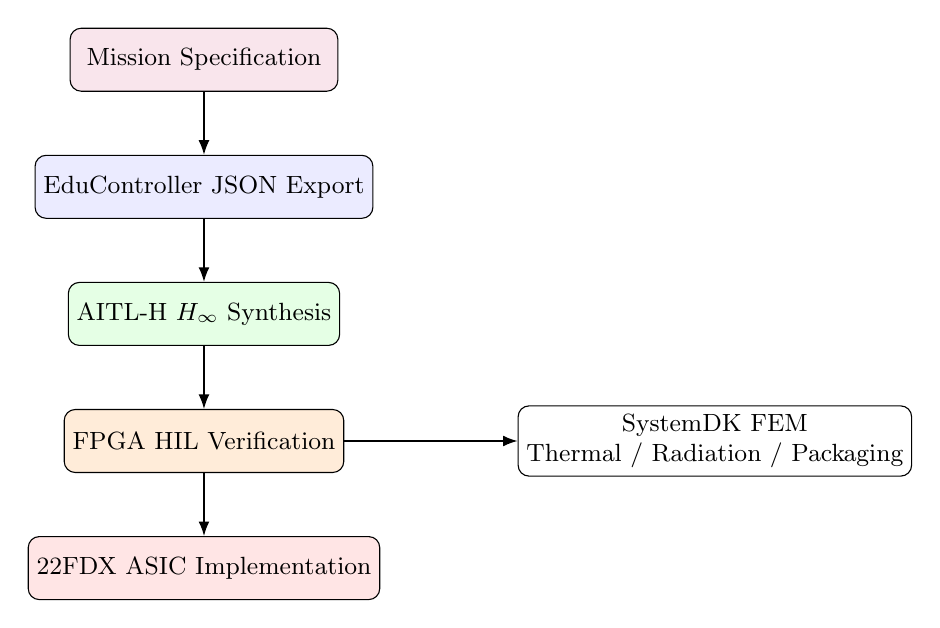
\begin{tikzpicture}[node distance=8mm]
  \node[midbox, fill=purple!10] (spec) {Mission Specification};
  \node[midbox, fill=blue!8, below=of spec] (json) {EduController JSON Export};
  \node[midbox, fill=green!10, below=of json] (synth) {AITL-H $H_\infty$ Synthesis};
  \node[midbox, fill=orange!15, below=of synth] (hil) {FPGA HIL Verification};
  \node[midbox, fill=red!10, below=of hil] (asic) {22FDX ASIC Implementation};

  \node[midbox, right=22mm of hil] (fem) {SystemDK FEM\\Thermal / Radiation / Packaging};

  \draw[line] (spec) -- (json);
  \draw[line] (json) -- (synth);
  \draw[line] (synth) -- (hil);
  \draw[line] (hil) -- (asic);
  \draw[line] (hil.east) -- (fem.west);
\end{tikzpicture}
\caption{End-to-end flow: Mission Spec $\to$ JSON (EduController) $\to$ AITL-H $\to$ FPGA HIL $\to$ FEM $\to$ ASIC.}
\label{fig:flow}
\end{figure}

% ---------- System Architecture ----------
\section{System Architecture}
AITL consists of three layers:
\begin{itemize}
  \item \textbf{Robust Core}: $H_\infty$/MPC/SMC controllers for ultra-robust stability.
  \item \textbf{FSM Supervisor}: mode switching (Safe/Nominal/Recovery) with FDI/FDII for fault management.
  \item \textbf{AI Adaptor}: long-term re-identification and drift compensation.
\end{itemize}

The tri-NVM hierarchy ensures persistence: SRAM for execution, MRAM for logs/code with ECC scrubbing and dual slots, and FRAM for safe boot and FSM states. The SoC target is 22\,nm FD\!SOI hardened against radiation and temperature stress.

% ---------- Fig.2 Architecture ----------
\begin{figure*}[t]
\centering
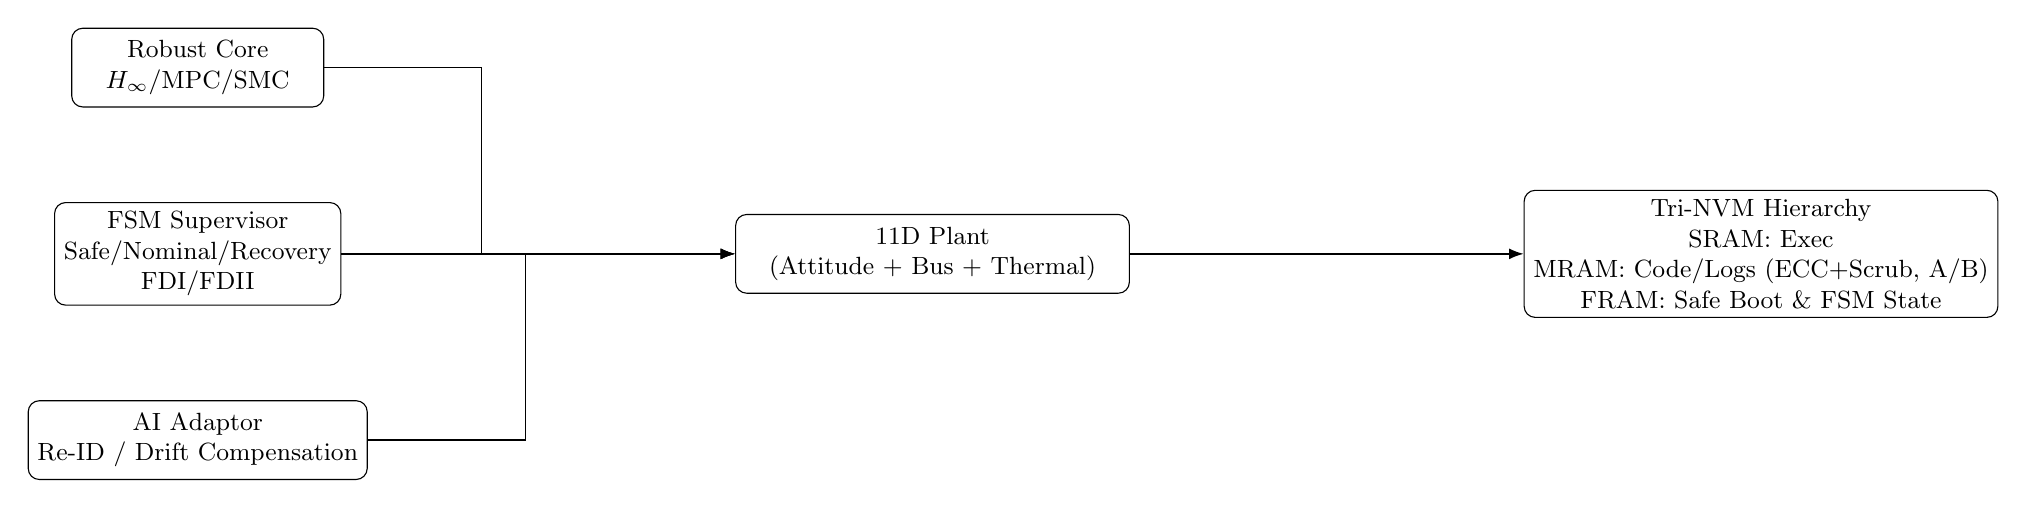
\begin{tikzpicture}[
  node distance=12mm and 15mm,
  box/.style={draw, rounded corners, align=center, minimum width=32mm, minimum height=10mm, font=\small},
  line/.style={-Latex, line width=0.5pt}
]

% 左カラム
\node[box] (core) {Robust Core\\$H_\infty$/MPC/SMC};
\node[box, below=of core] (fsm) {FSM Supervisor\\Safe/Nominal/Recovery\\FDI/FDII};
\node[box, below=of fsm] (ai) {AI Adaptor\\Re-ID / Drift Compensation};

% 中央プラント
\node[box, right=50mm of fsm, minimum width=50mm] (plant) {11D Plant\\(Attitude + Bus + Thermal)};

% 右カラム Tri-NVM
\node[box, right=50mm of plant, minimum width=48mm] (nvm) {Tri-NVM Hierarchy\\
SRAM: Exec\\MRAM: Code/Logs (ECC+Scrub, A/B)\\FRAM: Safe Boot \& FSM State};

% 矢印(水平直線)
\draw[line] (core.east) -- ++(20mm,0) |- (plant.west);
\draw[line] (fsm.east) -- ++(20mm,0) -- (plant.west);
\draw[line] (ai.east) -- ++(20mm,0) |- (plant.west);

\draw[line] (plant.east) -- (nvm.west);

\end{tikzpicture}
\caption{AITL on Space architecture with Robust Core, FSM Supervisor, AI Adaptor, and Tri-NVM hierarchy.}
\label{fig:arch}
\end{figure*}

% ---------- Mathematical Model ----------
\section{Mathematical Model and $H_\infty$ Design}
We consider an 11D discrete-time state-space plant coupling attitude (6), power bus (2), and thermal nodes (3):
\begin{align}
  x_{k+1} &= A x_k + B u_k + E w_k, \\
  y_k &= C x_k + D u_k + v_k,
\end{align}
where $w_k$ and $v_k$ denote disturbance and noise. The model extends to 20D by including translational axes and bias states.

Weights $(W_1,W_2,W_3)$ shape sensitivity, control effort, and complementary sensitivity. EduController outputs them as JSON; AITL-H synthesizes $K$ with robustness margins, mapped to fixed-point FPGA/ASIC.

% ---------- Fig.3 Control Loop ----------
\begin{figure}[t]
\centering
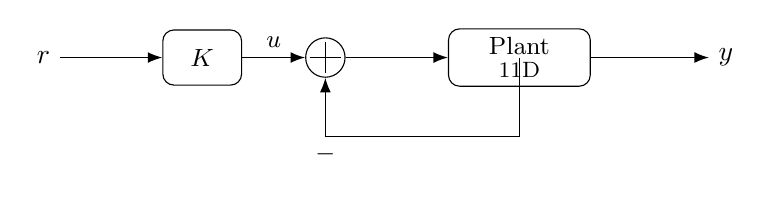
\begin{tikzpicture}[node distance=10mm]
  \node[smallbox, minimum width=10mm] (K) {$K$};
  \node[circle, draw, minimum size=5mm, right=8mm of K] (sum) {};
  \draw (sum) +(-2mm,0) -- +(2mm,0);
  \draw (sum) +(0,-2mm) -- +(0,2mm);
  \node[smallbox, right=13mm of sum, minimum width=18mm] (P) {\shortstack{Plant\\\footnotesize 11D}};
  \node[right=15mm of P] (y) {$y$};
  \node[left=13mm of K] (r) {$r$};
  \draw[line] (r) -- (K);
  \draw[line] (K) -- node[above]{\small $u$} (sum);
  \draw[line] (sum) -- (P);
  \draw[line] (P) -- (y);
  \draw[line] ($(P.south)!0.5!(P.north)$) |- ++(0,-10mm) -| node[below]{\small $-$} (sum.south);
\end{tikzpicture}
\caption{Closed-loop system for $H_\infty$ mixed-sensitivity synthesis on the 11D plant.}
\label{fig:loop}
\end{figure}

% ---------- Verification ----------
\section{Verification Pipeline}
FPGA HIL injects SEUs and outages, measuring safe-mode entry $< \SI{1}{s}$, recovery $\ge 99\%$, and ECC scrubbing efficiency. SystemDK FEM validates thermal/radiation stress, ensuring packaging reliability before ASIC tape-out.

% ---------- Conclusion ----------
\section{Conclusion}
AITL on Space combines robust control, supervisory safety, AI re-identification, and hardened memory. The proposed end-to-end flow—from mission specification to ASIC—provides a reproducible methodology for resilient autonomy in long-duration space missions.

% ---------- References ----------
\begin{thebibliography}{99}
\bibitem{doyle}
J.\,C.~Doyle, B.\,A.~Francis, and A.\,R.~Tannenbaum,
\emph{Feedback Control Theory}. Macmillan, 1992.

\bibitem{colinge}
J.-P.~Colinge, \emph{Silicon-on-Insulator Technology: Materials to VLSI}, 3rd~ed. Springer, 2004.

\bibitem{wolf}
W.~Wolf, \emph{FPGA-Based System Design}. Prentice Hall, 2004.

\bibitem{rabaey}
J.~M.~Rabaey, A.~Chandrakasan, and B.~Nikolic,
\emph{Digital Integrated Circuits: A Design Perspective}, 2nd~ed. Prentice Hall, 2003.
\end{thebibliography}

% ---------- Biography ----------
\section*{Author Biography}
Shinichi Samizo received the M.S.\ degree in Electrical and Electronic Engineering from Shinshu University, Japan. He worked at Seiko Epson Corporation as an engineer in semiconductor memory and mixed-signal device development, and contributed to inkjet MEMS actuators and PrecisionCore printhead technology. He is currently an independent semiconductor researcher focusing on process/device education, memory architecture, and AI system integration. Contact: \texttt{shin3t72@gmail.com}.
\end{document}
